\documentclass[11pt,a4paper]{article}
\usepackage[margin=2.3cm]{geometry}
\usepackage{amsmath,amssymb,bm,graphicx,booktabs,array,enumitem,xcolor,hyperref,float}

\hypersetup{colorlinks,linkcolor=blue!60!black,urlcolor=blue!60!black}
\setlength{\parskip}{4pt}
\title{\vspace{-1.2cm}The MLP of $t$ and the Fourier MLP:\\ what they are and where the parameter counts come from}
\author{Note for the paper meeting, 6 November 2026 (Joy)}
\date{}
\begin{document}
\maketitle
\vspace{-0.8cm}
\noindent\textit{Purpose.} Nadia asked (i) over how many runs the means are taken, (ii) whether $h=1$ in all one-hidden-layer experiments, and (iii) what the Fourier MLP is and how the parameter counts follow from $w$ and $W$, ``which is a matrix, but you multiply by $t$''. Section~1 answers (i) and (ii) in a few lines; the rest is (iii), from the shapes of the matrices to why the Fourier version works. Every number quoted is taken from the fit records of the study (\texttt{approx\_study/fits}).

\section{Runs and $h$}
\textbf{Runs.} Each neural model (KAN~[1,1], KAN~[1,$h$,1], MLP of $t$, Fourier MLP) is fitted three times, with seeds 0, 1, 2, on identical data; tables give the mean of the three, the Excel file also the sample standard deviation. A seed changes only the random starting point (initial weights; for the Fourier MLP also the frequencies drawn), never the data, budget, optimiser or number of steps. So the sd measures sensitivity to initialisation. For KAN~[1,1] it is $0$ to eight decimals, because that model is a least-squares problem with one minimiser (Section~5); for the MLPs it is $10^{-3}$--$10^{-2}$, because tanh networks have many local minima.

\textbf{$h$.} No, $h$ is the hidden width of KAN~[1,$h$,1] and is set per budget: $h=1,1,2,5,10$ for $N^*=15,30,60,120,240$. With grid size 3 and cubic splines each edge has $3+3=6$ spline coefficients, 2 scale weights and 4 (dormant) symbolic parameters, 12 in all, and [1,$h$,1] has $2h$ edges, so $N=24h$. The smallest network ($h=1$, $N=24$) already exceeds the 15 and 30 budgets, so those two rows use the same fit and show identical numbers; at 60 we use $h=2$ ($N=48$) rather than $h=3$ ($N=72$); 120 and 240 are exact.

\section{The MLP of $t$, with the shapes written out}
The network in Eq.~(6) of the paper takes the single number $t\in[0,1]$ and returns a single number $f(t)$:
\begin{equation}
f(t)=\bm W_3\,\tanh\!\bigl(\bm W_2\,\tanh(\bm W_1\,t+\bm b_1)+\bm b_2\bigr)+b_3 .
\label{eq:mlp}
\end{equation}
Read inside-out, with $w$ the number of neurons in each hidden layer:
\begin{center}
\renewcommand{\arraystretch}{1.25}
\begin{tabular}{llll}
\toprule
step & formula & shape of the result & parameters used \\
\midrule
input & $t$ & $1\times1$ (a scalar) & -- \\
layer 1 & $\bm z_1=\bm W_1 t+\bm b_1$ & $w\times1$ & $\bm W_1\in\mathbb R^{w\times1}$ ($w$), $\bm b_1\in\mathbb R^{w}$ ($w$)\\
activation & $\bm a_1=\tanh(\bm z_1)$ (entrywise) & $w\times1$ & -- \\
layer 2 & $\bm z_2=\bm W_2\bm a_1+\bm b_2$ & $w\times1$ & $\bm W_2\in\mathbb R^{w\times w}$ ($w^2$), $\bm b_2\in\mathbb R^{w}$ ($w$)\\
activation & $\bm a_2=\tanh(\bm z_2)$ & $w\times1$ & -- \\
output & $f=\bm W_3\bm a_2+b_3$ & $1\times1$ & $\bm W_3\in\mathbb R^{1\times w}$ ($w$), $b_3\in\mathbb R$ (1)\\
\bottomrule
\end{tabular}
\end{center}
So $\bm W_1$ is a matrix only in the formal sense: it has $w$ rows and \emph{one} column, i.e.\ it is a column vector $\bm w_1=(w_{11},\dots,w_{w1})^{\!\top}$, and ``$\bm W_1 t$'' is that vector scaled by the number $t$. The first hidden neuron computes $\tanh(w_{11}t+b_{11})$, the second $\tanh(w_{21}t+b_{21})$, and so on: $w$ different S-shaped curves of $t$, each with its own slope and position. The second layer mixes those $w$ curves with a full $w\times w$ matrix and bends the mixtures again; the output layer takes one weighted sum. Writing the first layer as $\bm w_1 t$ (lower case) in the paper would make this explicit; it changes nothing else.

Adding the entries of the last column gives the count used in Section~4.3 and Table~3:
\begin{equation}
N_{\text{MLP}}=\underbrace{w+w}_{\text{layer 1}}+\underbrace{w^2+w}_{\text{layer 2}}+\underbrace{w+1}_{\text{output}}=w^2+4w+1 .
\end{equation}
For $w=2,4,6,9,14$ this is $13,33,61,118,253$, the nearest achievable values to the budgets $15,30,60,120,240$; the count is quadratic in $w$, so it cannot be made to land exactly.

\section{The Fourier MLP: the same network, a different input}
The only change is what goes in. Instead of the scalar $t$ we feed the vector
\begin{equation}
\bm\gamma(t)=\bigl[\sin(2\pi b_1 t),\dots,\sin(2\pi b_m t),\;\cos(2\pi b_1 t),\dots,\cos(2\pi b_m t)\bigr]^{\!\top}\in\mathbb R^{2m},
\qquad b_j\sim\mathcal N(0,\sigma^2),
\label{eq:fourier}
\end{equation}
with $\sigma=6$ and the $m$ frequencies $b_j$ drawn once (per seed) and then frozen: they are not trained and not counted. Because the input now has $2m$ entries, the first matrix must have $2m$ columns, $\bm W_1\in\mathbb R^{w\times 2m}$, and that is the whole difference. The table becomes:
\begin{center}
\renewcommand{\arraystretch}{1.25}
\begin{tabular}{lll}
\toprule
layer & shapes & parameters \\
\midrule
input & $\bm\gamma(t)\in\mathbb R^{2m}$ & 0 (frequencies fixed)\\
layer 1 & $\bm W_1\in\mathbb R^{w\times2m}$, $\bm b_1\in\mathbb R^{w}$ & $2mw+w$\\
layer 2 & $\bm W_2\in\mathbb R^{w\times w}$, $\bm b_2\in\mathbb R^{w}$ & $w^2+w$\\
output & $\bm W_3\in\mathbb R^{1\times w}$, $b_3\in\mathbb R$ & $w+1$\\
\bottomrule
\end{tabular}
\end{center}
\begin{equation}
N_{\text{FMLP}}=2mw+w+w^2+w+w+1=w^2+(2m+3)w+1 .
\end{equation}
Two integers can now be adjusted, which is why this model gets closer to the budgets than the plain MLP: $(m,w)=(2,2),(2,3),(4,4),(6,6),(8,9)$ give $N=19,31,61,127,253$. A quick check of one row: $(4,4)$ gives $2\cdot4\cdot4+4+16+4+4+1=61$, the number in Table~3.

\begin{figure}[H]\centering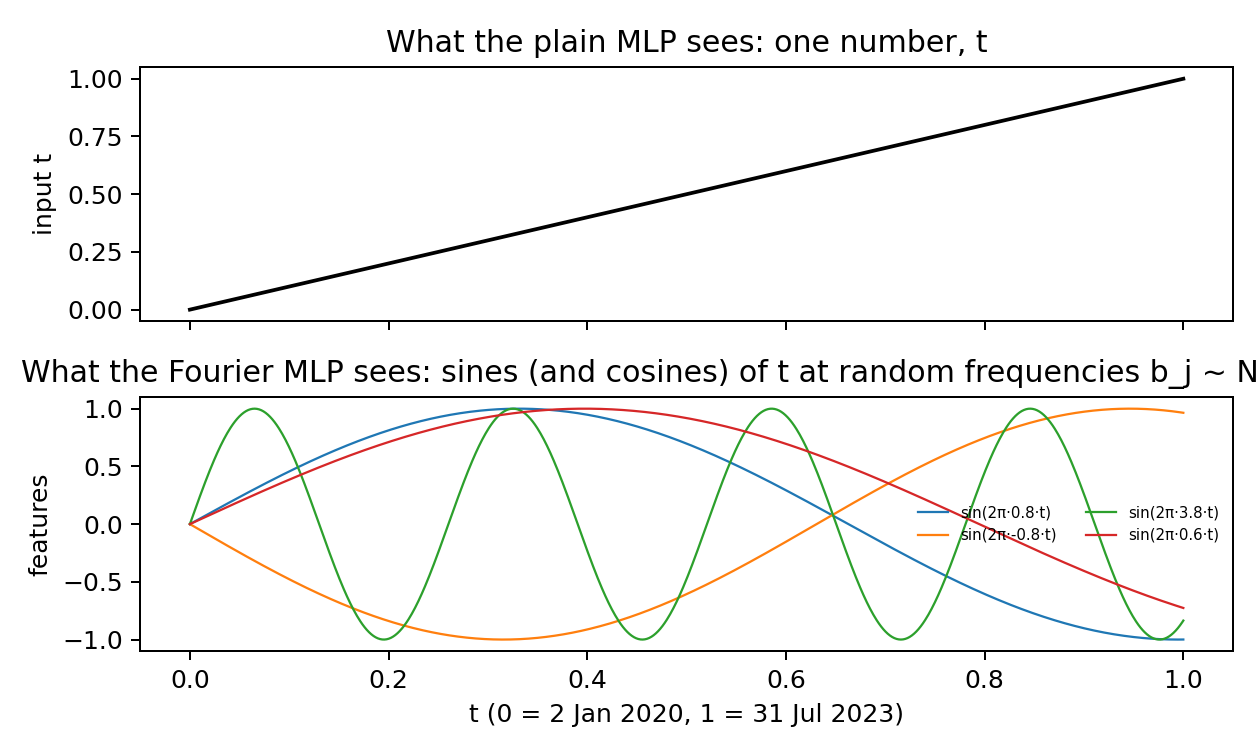
\includegraphics[width=.92\textwidth]{fig_features.png}
\caption{Top: the plain MLP receives one number, $t$. Bottom: the Fourier MLP receives $2m$ numbers, the sines (shown) and cosines of $t$ at $m$ random frequencies; here four draws from $\mathcal N(0,6^2)$. The frequencies are in cycles per full series, so $b=6$ means six oscillations over the 3.5 years, a period of about seven months.}
\end{figure}

\section{Why feed sines and cosines? Spectral bias}
A tanh network trained by gradient descent is lazy in a specific way: it fits the slowly varying part of the target quickly and acquires fast wiggles only very slowly. Rahaman et al.\ (ICML 2019) named this \emph{spectral bias} and showed it both empirically and for shallow networks analytically: in a Fourier decomposition of the network's output, the low-frequency components are learned orders of magnitude faster than the high-frequency ones. A price path is nothing but wiggles on top of a trend, so a plain MLP of $t$ spends its 20{,}000 steps mostly getting the trend right (Figure~\ref{fig:bias}, right).

Tancik et al.\ (NeurIPS 2020) showed that passing the input through random Fourier features, Eq.~\eqref{eq:fourier}, removes the handicap: the network no longer has to manufacture oscillations from S-curves, it is handed oscillations of many pitches and only has to learn how to combine them. The mathematics behind it is that the composition ``network of $\bm\gamma(t)$'' has a kernel whose spectrum is set by the distribution of the $b_j$, so choosing $\sigma$ chooses which frequencies the model finds easy. An analogy: the plain MLP draws the curve with a soft pencil that can only make broad strokes; the Fourier MLP is given a set of tuning forks of random pitch and asked to mix them.

\begin{figure}[H]\centering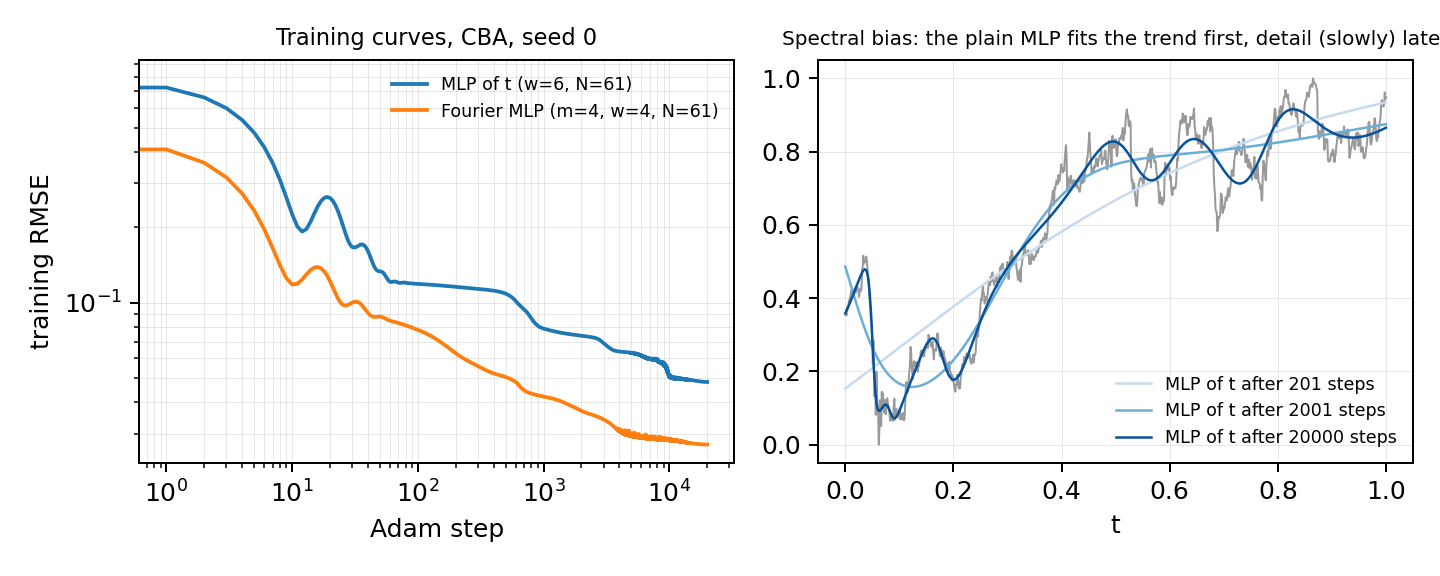
\includegraphics[width=.98\textwidth]{fig_bias.png}
\caption{Left: training RMSE against Adam step for the two 61-parameter networks on CBA (seed 0; the curves end at $0.0482$ and $0.0271$, exactly the values in the fit records). Right: the plain MLP's output after 201, 2001 and 20{,}000 steps: the trend is captured almost immediately, detail arrives slowly and incompletely.}
\label{fig:bias}
\end{figure}

\begin{figure}[H]\centering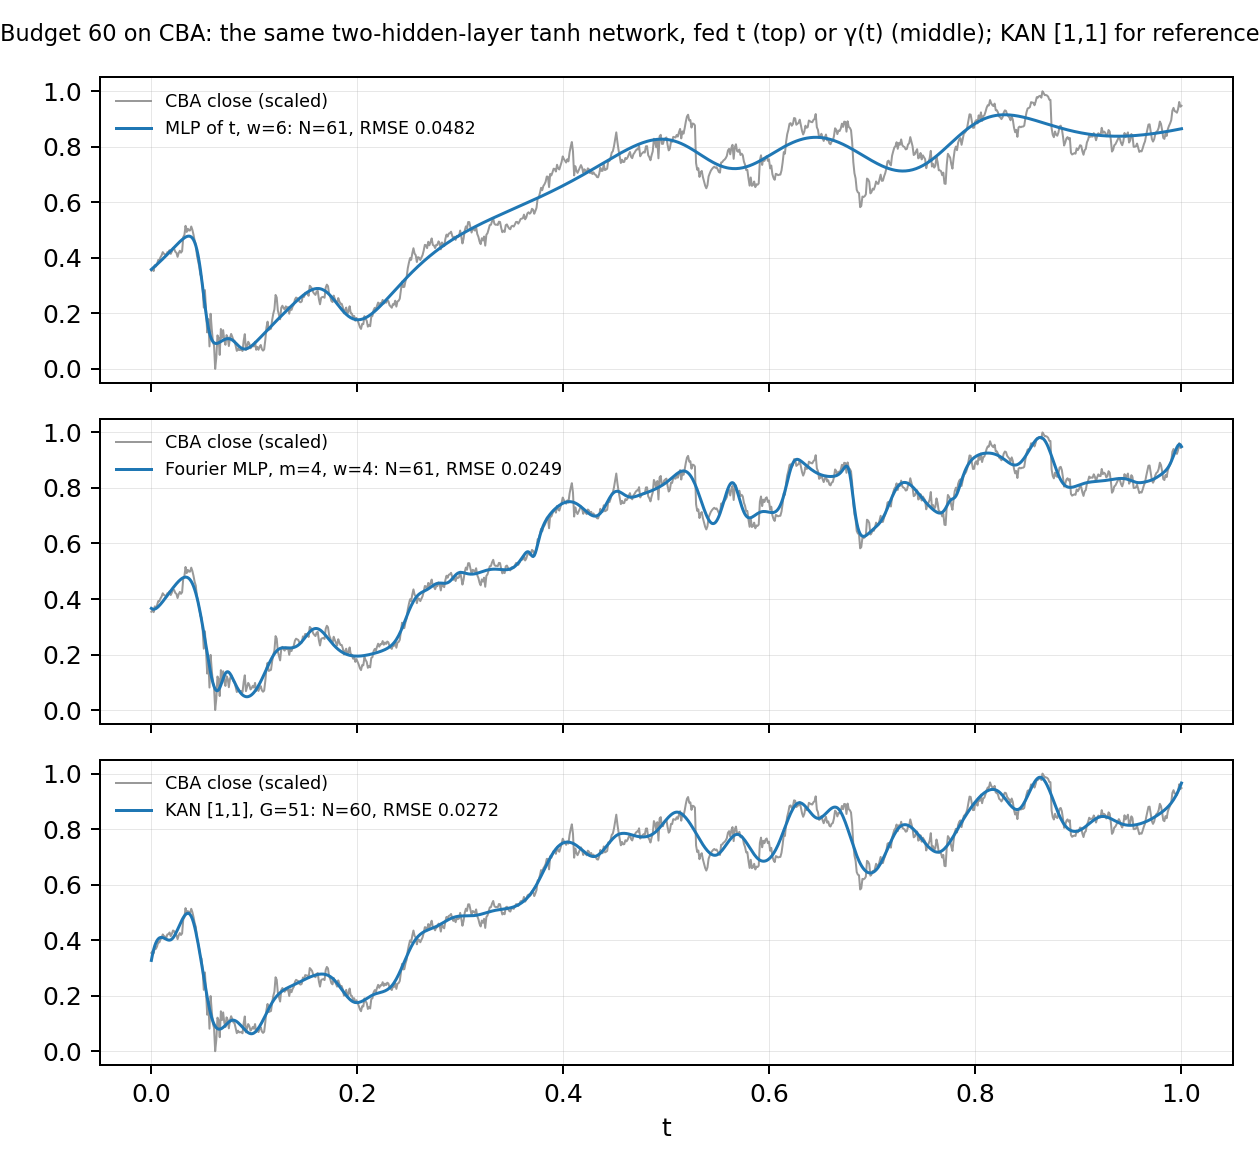
\includegraphics[width=.9\textwidth]{fig_fits.png}
\caption{Budget 60 on CBA, best of three seeds. Top: MLP of $t$ ($w=6$, $N=61$, RMSE $0.0482$). Middle: Fourier MLP ($m=4$, $w=4$, $N=61$, RMSE $0.0258$). Bottom: KAN~[1,1] ($G=51$, $N=60$, RMSE $0.0272$). Same architecture top and middle; the only change is the input.}
\end{figure}


\section{Why the Fourier MLP and the KAN~[1,1] end up so close}
A KAN~[1,1] is a single learnable function of one variable,
$f(t)=w_b\,\mathrm{silu}(t)+w_s\sum_{i}c_i B_i(t)$, with $B_i$ the cubic B-splines on $G$ equal subintervals of $[0,1]$. For fixed knots this is linear in the $c_i$, so fitting it is an ordinary least-squares problem with a unique solution; that is why its sd over seeds is zero and why it coincides with a classical least-squares spline. Its parameter count is $N=G+9$: $G+3$ coefficients, 2 scale weights, and the 4 symbolic-branch parameters PyKAN keeps on every edge (unused here but trainable, hence counted).

Both the spline and the Fourier MLP are, in effect, expansions in a fixed family of basis functions (local bumps versus global waves), so at equal parameter counts they reach similar accuracy once the Fourier network has enough frequencies to cover the detail. The plain MLP has to build its own basis out of a handful of S-curves and cannot keep up. Table~\ref{tab:cba} shows the three side by side.

\begin{table}[H]\centering
\caption{CBA, RMSE in scaled $[0,1]$ units, mean over 3 seeds (actual $N$ in brackets).}
\label{tab:cba}
\begin{tabular}{lccc}
\toprule
budget $N^*$ & MLP of $t$ & Fourier MLP & KAN [1,1]\\
\midrule
15  & 0.0753 (13) & 0.0842 (19) & 0.0707 (15)\\
30  & 0.0634 (33) & 0.0579 (31) & 0.0464 (30)\\
60  & 0.0566 (61) & 0.0258 (61) & 0.0272 (60)\\
120 & 0.0531 (118) & 0.0177 (127) & 0.0172 (120)\\
240 & 0.0419 (253) & 0.0130 (253) & 0.0131 (240)\\
\bottomrule
\end{tabular}
\end{table}

\section{Questions that may follow, briefly}
\begin{description}[leftmargin=0pt,itemsep=3pt]
\item[Why is the Fourier MLP worse than the plain MLP at budgets 15 and 30?] With $m=2$ it has only four waves at random pitches and almost no width ($w=2,3$) to correct a poor draw; its sd there is the largest in the study ($\pm0.037$ at CBA, 15). From 60 parameters on the ordering reverses and stays reversed on all three assets.
\item[Was $\sigma$ tuned?] No; $\sigma=6$ was fixed before the runs. One spot check afterwards (CBA, 240) gave $0.0271$ at $\sigma=6$ and $0.0257$ at $\sigma=20$, so a tuned Fourier MLP would be slightly better still. This is a discussion point, not a configuration detail.
\item[Why is $\sigma$ in those units?] $t\in[0,1]$ spans the whole series, so $b_j$ is in cycles per 3.5 years; $|b_j|\le 12$ (two standard deviations) corresponds to periods of three and a half months or longer. Higher $\sigma$ lets the model reach shorter periods.
\item[Why does the KAN~[1,$h$,1] not share the KAN~[1,1]'s advantage?] It spends $24h$ parameters on $2h$ edges with only $G=3$ intervals each, so every edge is a coarse spline and detail must come from composing coarse pieces; and the problem is no longer convex, so 80 L-BFGS steps are not always enough (CBA, 120: $0.0447$ at 80 steps, about $0.037$ at 320--640). Both points favour [1,1].
\item[80 L-BFGS steps against 20{,}000 Adam steps: fair?] Not symmetric, and the paper says so. KAN~[1,1] converges by 20 steps, so more would not change it; the MLPs at 20{,}000 are slightly undertrained (CBA, 240: $0.0393\to0.0363$ at 40{,}000), by less than the gap to the KAN.
\item[Units in dollars?] Errors are in each asset's Min--Max scaled close, $1.0$ = its full price range. TSLA (close 24.08--409.97): an RMSE of $0.03$ is about \$11.6; LLY (119.05--468.98): about \$10.5. (CBA's raw series is not in the current data set, only the scaled one.)
\item[Where were the fits run?] In a Linux CPU sandbox, not on the Zenbook of the hardware table. Errors reproduce exactly (seeded, CPU); the seconds will differ. Either rerun on the laptop or qualify the caption.
\end{description}

\vspace{4pt}\noindent\textbf{References.}\ N.~Rahaman et al., \emph{On the spectral bias of neural networks}, ICML 2019 (PMLR 97:5301--5310).\ M.~Tancik et al., \emph{Fourier features let networks learn high frequency functions in low dimensional domains}, NeurIPS 2020.\ Z.~Liu et al., \emph{KAN: Kolmogorov--Arnold Networks}, 2024 (arXiv:2404.19756).\ R.~Yu, W.~Yu, X.~Wang, \emph{KAN or MLP: a fairer comparison}, 2024 (arXiv:2407.16674).
\end{document}
